%# -*- coding: utf-8-unix -*-
%%==================================================
%% chapter02.tex for SJTU Master Thesis
%% based on CASthesis
%% modified by wei.jianwen@gmail.com
%% Encoding: UTF-8
%%==================================================


\chapter{基于规范的入侵检测设计}
\label{chap:spec detection}

\section{引言}
\label{sec:intro}
在上一章节中我们讨论了如何对控制器与物理设备交互的输入输出信号进行检测保护,防御对象系统主要是故障和异常数据注入攻击,为此我们还专门设计错误序列注入攻击对其进行仿真验证。但是对控制器本身尤其是PLC这种可编程控制器,由于它们在整个控制系统中发挥至关重要的作用,近年来正成为对物理设备损坏性攻击的有吸引力的目标。最为典型的Stuxnet病毒可以向PLC上传恶意代码,以物理损坏他们控制的离心机。更有研究发现,PLC控制器不仅容易被端口扫描,而且还可以被修改控制系统特定协议和被访问诊断系统。这些易受攻击的互联网控制器被计算机搜索引擎暴露,例如Shodan。所以对可编程控制器本身控制程序和指令的保护并使其免受恶意代码注入的保护也同样重要。本章我们提出了基于规范的的入侵检测来应对控制器的恶意代码注入攻击,只有经过验证合法的程序和指令才能操作系统或控制服务器上传到指定的可编程控制器设备中。

\section{入侵检测方案概述}
\label{sec:list}

本文我们采用PLC作为待检测可编程控制器,检测机制作为外部单独的功能处理器BITS(Bump-in-the-wire)模式放置在控制系统网络和PLC之间。对于任何等待上传到工业设备的PLC代码,将被拦截并验证由过程安全工程师定义的一整套安全规范(safety properties),安全特性的示例包括数字设备参数(例如最大驱动速度和加速度)和安全互锁的界限并确保不发生物理上冲突的事件。图\ref{fig21}展示了基于规范入侵检测机制的基本过程,首先将PLC代码(IL code)格式化整理并通过IL2boolIL算法转换为中间语言,我们定义为布尔逻辑指令表代码(Boolean IL code),旨在使抽象程序逻辑清晰更具一般性。然后布尔逻辑指令表代码通过模板实例化(Template Instantiate
)过程被迭代地执行转化,将通用模板代码实例化为验证工具NuSMV输入程序。前面两步是对PLC程序的形式化建模过程,接下来我们给出验证过程。我们通过将得到的形式化代码模型(NuSMV code)输入到验证工具NuSMV逐个地检查我们的安全规范。每个布尔规范表示有限状态机中的安全属性是否为真,如果存在任何可达的路径其属性为假,则会给出相应的反例并证明存在安全违规不能而且上传到PLC设备中。

\begin{figure}[!htb]
\centering
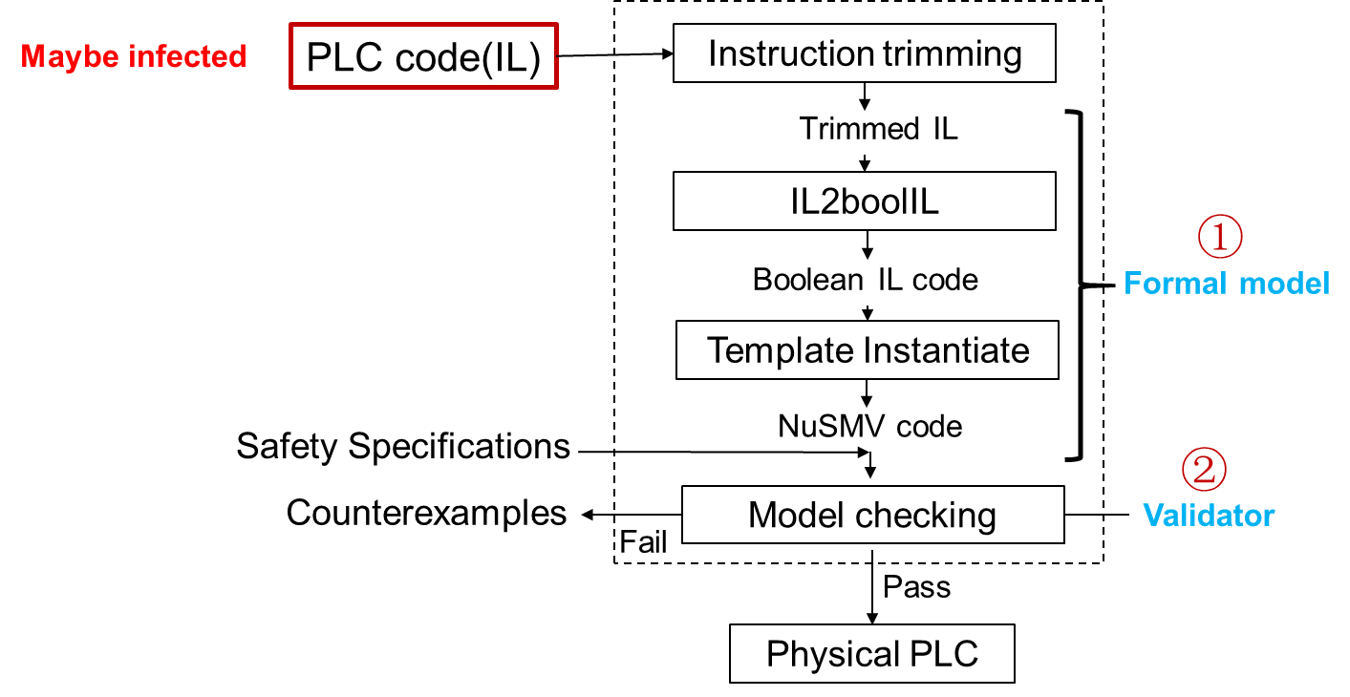
\includegraphics[scale=0.49]{spec/flowchart_spec.png}
\caption{基于规范的入侵检测流程图}
\label{fig21}
\end{figure}

\section{系统建模和入侵检测设计}
\label{sec:matheq}

\subsection{PLC指令表程序介绍}

指令表程序(Instruction  List,IL)是一种较老的PLC编程语言,它使用类似于计算机的一些助记符记号来表示PLC的操作功能,并根据相应的词法和语法写入每一行程序,以实现工业要求的控制目标和运算处理。

指令表程序具有以下特点:

\begin{itemize}
	\item 每条指令包含明确的功能而且变量之间的逻辑关系清晰。 
	\item 类似于汇编语言,与其他四种编程语言相比更适合现有的程序验证方法。 
	\item 系统执行效率高。
	\item 和其他四种编程语言可以直接对应。
\end{itemize}

因此,为了真正了解PLC程序变量之间的逻辑关系,实现PLC程序的形式验证,首先我们必须掌握指令表程序,这也是指令表程序成为我们研究对象的重要原因。虽然国际电工委员会在IEC61131-3中定义了国际标准的指令表程序,但为了提高系统效率的实际应用,以西门子、洛克威尔和三菱PLC为代表的厂商都发展自己的具体指令表程序规范。尽管每个公司对于指令表程序具有不同的命名约定,但是这些指令表程序在逻辑级上的含义是相同的。由于我们更多关注指令表语义的逻辑,PLC厂商这个因素不会影响我们的检测研究。本文将以西门子的指令程序语句表(Statement  List,STL)为对象开始相关研究工作。

在西门子S7-200指令系统中,可以分为基本指令和应用指令。所谓的基本指令,最初是指代替传统继电器控制系统所要求的指令。随着PLC的功能越来越强大,越来越多的指令被涉及,基本指令的内容也在逐步地扩展。 它包括基本逻辑指令、操作指令、数据处理指令、表函数指令和转换指令。基本逻辑指令包括基本位操作指令、比较指令、定时器指令、逻辑堆栈指令和计数器指令。基本逻辑指令构成指令集的基本逻辑运算功能,是所有其他指令应用的基础。因此,本文选择基本逻辑指令作为建模对象进行研究工作。表\ref{spec:il}展示了我们涉及到的常用的基本指令。

%\newcommand{\tabincell}[2]{\begin{tabular}{@{}#1@{}}#2\end{tabular}}
\begin{table}[!htp]
\centering
\caption{IL指令表基本指令表}
\label{spec:il}
\begin{tabular}{|p{2cm}<{\centering}|p{3cm}<{\centering}|p{8cm}<{\centering}|}
\hline
指令 & 指令类别 & 指令描述 \\
\hline
\end{tabular}
\begin{tabular}{|p{2cm}|p{3cm}|p{8cm}|}
\hline
LD & 逻辑指令 & 装载指令,用于网络块逻辑运算的开始。 \\
\hline
LDN & 逻辑指令 & 装载反指令,用于网络块逻辑运算的开始。 \\
\hline
A & 逻辑指令 & 与指令,表示用串联的形式连接单个常开触点。 \\
\hline
AN & 逻辑指令 & 与反指令,表示用串联的形式连接单个常闭触点。 \\
\hline
O & 逻辑指令 & 或指令,表示用并联的形式连接单个常开触点。 \\
\hline
ON & 逻辑指令 & 或反指令,表示用并联的形式连接单个常闭触点。 \\
\hline
S/R & 逻辑指令 & 置位和复位指令。 \\
\hline
OLD & 逻辑堆栈指令 & 或块指令,表示用并联的形式连接串联电路块。 \\
\hline
ALD & 逻辑堆栈指令 & 与块指令,表示用串联的形式连接串联电路块。 \\
\hline
LPS & 逻辑堆栈指令 & 逻辑入栈指令,也称为分支电路开始指令。从堆栈角度看,LPS指令的功能是把栈顶值拷贝后存入堆栈。\\
\hline
LRD & 逻辑堆栈指令 & 逻辑读栈指令,从堆栈角度看,LRD将第二个堆栈值复制到堆栈顶部。堆栈没有被弹出,但堆栈顶部的旧数值会被破坏。
\\
\hline
LPP & 逻辑堆栈指令 & 逻辑出栈指令,从堆栈角度看,LPP将
将堆栈的一个数值弹出堆栈,第二个堆栈数值称为堆栈数值的新顶部。\\
\hline
TON & 逻辑定时器指令 & 接通延时定时器,表示对单一时间间隔进行定时控制。 \\
\hline
CTU & 逻辑计数器指令 & 增计数器,首次扫描其值为0,在计数脉冲输入端CU的每个上升沿计数器计数一次直到32767后停止计数,复位输入端有效值为0。 \\
\hline
JMP/LBL & 控制指令 & 跳转指令和标号指令,使主机可根据不同条件进行判断,选择不同的程序段执行程序 \\
\hline

\end{tabular}
\end{table}

\subsection{PLC程序的形式化建模}

\textbf{定义1:} IL程序网络(network)是由3元组迁移函数表示: \[ \mathcal{T_{IL}}=(C,c_0,\rightarrow) \] 其中
\begin{itemize}
	\item $C$ 是IL程序配置集
	\item $ c_0 $ 是IL程序初始配置集
	\item $ \rightarrow $ 是迁移关系
\end{itemize}
这里每一个IL程序配置$c\in C$可以由\[ c=(\sigma,e,E) \] 其中
\begin{itemize}
	\item $\sigma$ 是IL程序变量状态
	\item $ e $ 是IL程序网络中将要执行的变量
	\item $ E $ 是IL程序网络中未执行的变量集
\end{itemize}

因为没有标准的步骤来验证PLC程序,我们形式建模的目的是为了通过生成中间语言来更好地或直接转换为NuSMV输入程序。PLC程序的形式模型分为两个阶段。对于第一步,我们采用指令表(IL)作为我们的主要研究的PLC语言程序,并且我们需要在算法\ref{algo:boolil}中将IL代码转换为布尔逻辑代码(boolIL),即给出映射算法$\={h}: IL \rightarrow boolIL$使得对于IL程序中的每个将要执行的元素$e$都能映射到boolIL中的表示$a=\={h}(e)$。在网络中执行IL运算符的顺序由下一个映射决定:$2^{IL}\rightarrow IL$根据已经执行的元素集确定接下来执行哪个元素。而在boolIL中这一动作已由程序计数器执行并定义映射$p: boolIL\rightarrow IN$将程序中每一条指令$a$映射到它所在的行数$pc$。相应的我们给出boolIL语言的定义:

\textbf{定义2:} boolIL程序网络(network)是也由3元组迁移函数表示: \[ \mathcal{T}_{boolIL}=(B,b_0,\rightarrow) \] 其中
\begin{itemize}
	\item $B$ 是boolIL程序配置集
	\item $ b_0 $ 是boolIL程序初始配置集
	\item $ \rightarrow $ 是迁移关系
\end{itemize}
这里每一个IL程序配置$b\in B$可以由\[ b=(\sigma,a,pc) \] 其中
\begin{itemize}
	\item $\sigma$ 是boolIL程序变量状态
	\item $ a $ 是boolIL程序网络中将要执行的语句
	\item $ pc $ 是boolIL程序网络中$a$语句所在的程序行号
\end{itemize}

第一步的主要目的是在程序中从复杂的IL代码通过逐行解释上下文和语义获得二进制函数输出。算法\ref{algo:boolil}首先将完整的程序划分为多个程序块,然后将每个程序块划分为多个网络块部分并初始化所有的集合。其次,我们对每个逻辑和控制指令执行符号解释以获得二进制函数结果。最后,当实现所有IL程序时,每个结果将从存储器输出。

\begin{algorithm}[!htb]
\caption{IL2boolIL算法}
\label{algo:boolil}
\begin{algorithmic}[1]
\Require %算法的输入参数:Input  
IL程序;

\Ensure %算法的输出:Output  
boolIL程序$S_{x_{init}}$;  

\State 将完整程序划分成多个程序块$V'$并将每个程序块划分为多个网络块$F$
\State 初始化并设置$V'= 1,F=\emptyset$;
\For{each $j \in SUM_{所有网络块部分}$}
\Switch{第$j$个网络块部分}
\Case {$OP$部分}
\For{each $i \in SUM_{本网络块的总行数}$}
\Switch{第$i$行程序指令}
\Case {$LD$($LND$)}
\State 设置相应的变量值为初始值(取反)输入并存入内存; break;
\EndCase
\Case {$A$($AN$)}
\State 设置相应的变量值为(取反)输入与($\&$)上前一指令的运算结果并存入内存; break;
\EndCase
\Case {$O$($ON$)}
\State 设置相应的变量值为(取反)输入或($|$)上前一指令的运算结果并存入内存; break;
\EndCase
\Case {$TON/CTU/S/R$}
\State 定时器/计数器/置位/复位指令,需要进行抽象建模处理; break;
\EndCase
\EndSwitch
\EndFor
\EndCase
\Case {$ALD$($OLD$)}
\State 使前两个指令运算结果执行与$\&$(或$|$)操作并将执行结果入栈; break;
\EndCase
\Case {$LPS/LPD/LPP$}
\State 存入/读取/弹出堆栈中前一指令的运算结果; break;
\EndCase
\Case {$JMP/LBL$}
\State 控制指令,需要进行抽象建模处理; break;
\EndCase
\Case {$=$}
\State 输出内存中的最终结果; break;
\EndCase
\Default
\State Return $S_{x_{init}}$
\EndDefault
\EndSwitch
\EndFor
\State Return $S_{x_{init}}$
\end{algorithmic}
\end{algorithm}

从算法\ref{algo:boolil}我们看出有四类指令程序是无法直接进行解释执行的,因此我们需要对这四类指令进行抽象建模。

\begin{enumerate}
	\item $S/R$指令\\
	\begin{center}
	\framebox[250pt][c]{
	\parbox[c]{100pt}{
	\framebox[60pt][c]{IN}\\
	\makebox[60pt][c]{$\downarrow$}\\
	\makebox[60pt][c]{S/R Out}} $\Rightarrow \begin{cases} S: Out=IN\& Out\\R: Out=!(IN|Out)\end{cases}$ }
	\end{center}
	我们发现$S/R$有自锁的特性,即当$S$的输出$Out$为0时,不管其前面的程序集的输入$IN$为何值,其结果总为0,相应的$R$指令也有类似的特性。

	\item 控制指令$JMP$和$LBL$\\
	\begin{center}
	\framebox[350pt][c]{
	\parbox[c]{80pt}{
	\framebox[60pt][c]{X}\\
	\makebox[60pt][c]{$\downarrow$}\\
	\makebox[60pt][c]{JMP n}\\
	\makebox[60pt][c]{$\downarrow$}\\
	\framebox[60pt][c]{$Y_n(y_n)$}\\
	\makebox[60pt][c]{$\downarrow$}\\
	\makebox[60pt][c]{LBL n}\\
	\makebox[60pt][c]{$\downarrow$}} 
	$\Rightarrow$ $ Y_n=(Y_n \& (y_n|!X)) | (y_n\&X)  = \begin{cases} y_n,~~ if~X=1\\Y_n,~~ if X=0\end{cases}$
	}
	\end{center}
	这里的$X$是$JMP$指令的输入,$Y_n$是$LBL$指令的输入,$y_n$是$Y_n$的初始值。抽象建模后的$Y_n$的输出严格遵循控制指令的语义,即当$X=1$时,控制指令激活并跳过$JMP$和$LBL$之间的程序,$Y_n$的输出即为初始输出值$y_n$;当$X=0$也能得到类似的结论。
	\item 定时器指令TON\\
	如图\ref{fig22}所示,定时器的端口由输入$IN$、输出$Q$和定时时间$PT$组成,右上方的状态转移图描述了定时器执行过程中的三个状态迁移过程。初始状态$NR$输出$Q$为$false$,输入$IN$未激活置为0;当$IN$激活后但未达到时间要求时,迁移到第二状态$R$,此时输出$Q$仍为$false$;如果在未达到定时时间时,输入被置0则又会回到初始状态$NR$,一旦在激活状态且达到定时时间,定时器会到达它的第三状态$TO$,此时输出$Q$为$true$,如果输入又被置0则又会回到初始状态$NR$。这里要特别说明我们并没有模拟具体的时间,对于是否满足时间要求我们只给出$true$和$false$两个状态。为了便于理解,图的下方给出了简单的例子,定时器$T1$的运算结果由输入$In1$和定时时间状态$T1Ton$共同决定。
	\begin{figure}[!htb]
	\centering
	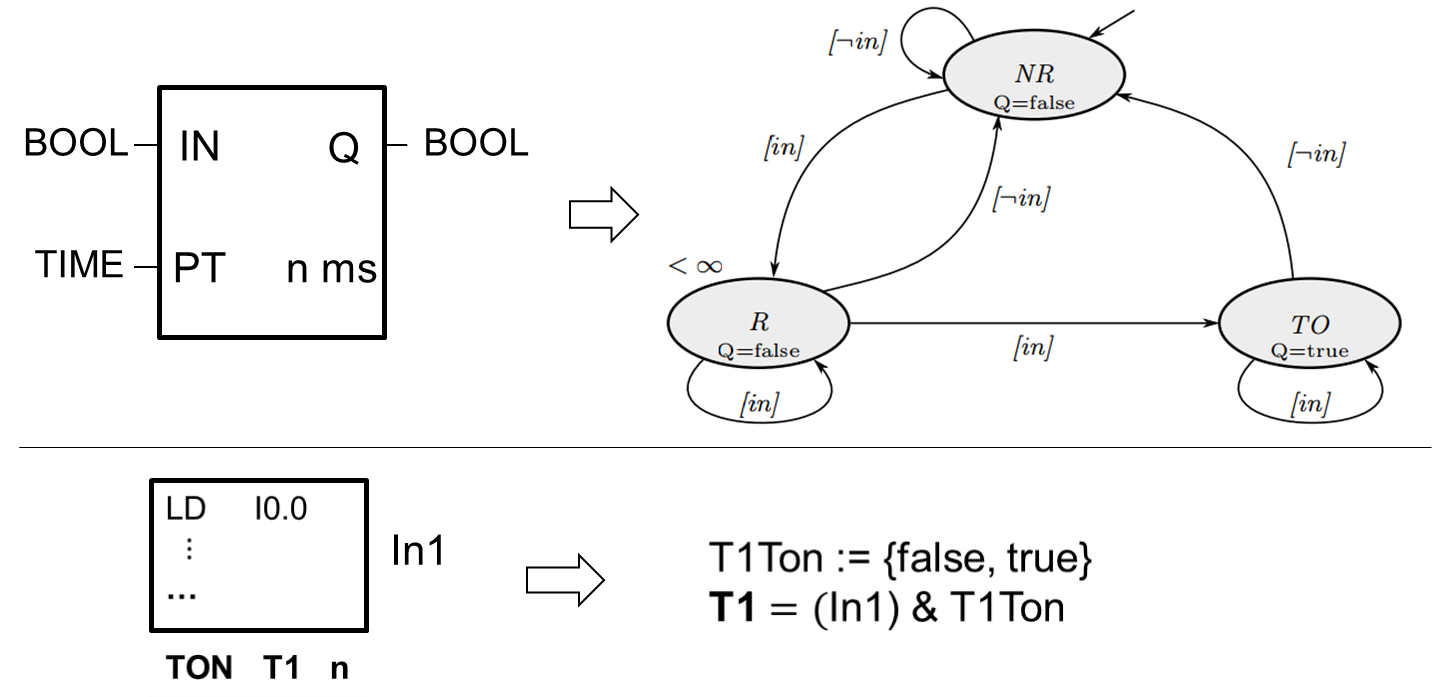
\includegraphics[scale=0.48]{spec/ton.png}
	\caption{TON指令的抽象建模}
	\label{fig22}
	\end{figure}


	\item 计数器指令$CTU$\\
	如图\ref{fig23}左上方所示,计数器的端口由输入$CU$、重置$R$、计数次数$PV$和输出端$Q$(单独的端口)组成,右上方的状态转移图描述了定时器执行过程中的四个状态迁移过程。初始状态输出$Q$为$false$,输入$CU$未激活置为0且重置$R=0$;当$IN$激活后且重置$R=0$但未达到计数次数要求时,迁移到第二种状态即激活状态,此时输出$Q$仍为$false$;如果在未达到计数次数时,输入被置0则又会回到初始状态,一旦在激活状态时未被重置且达到计数次数$N$,计数器会到达它的第三种状态即响应状态,此时输出$Q$为$true$,如果重置$R=0$则会到达第四种状态即重置状态,此时$Q=false$且$PV=0$被重置。为了便于理解,图的下方给出了简单的例子,计数器$C20$的运算结果由输入$C20CU$和计数次数状态$PV$共同决定。

	\begin{figure}[!htb]
	\centering
	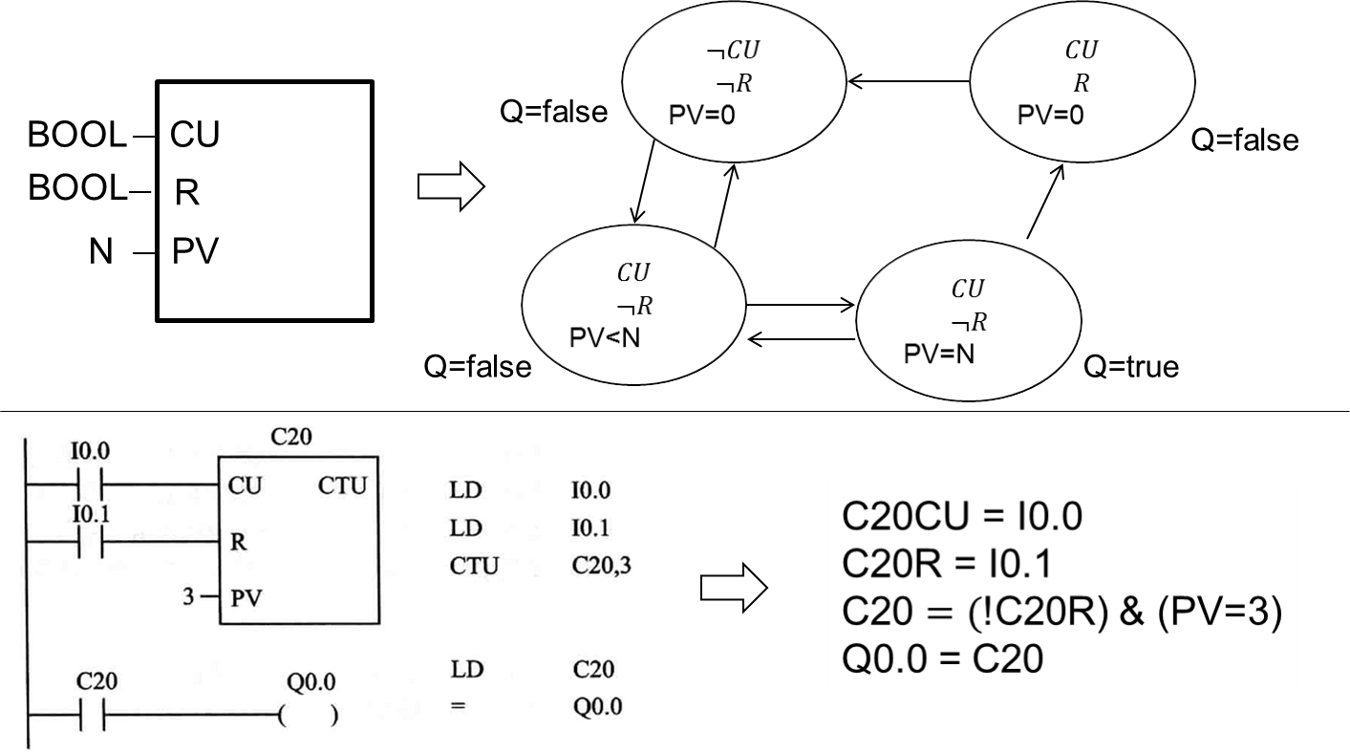
\includegraphics[scale=0.48]{spec/ctu.png}
	\caption{CTU指令的抽象建模}
	\label{fig23}
	\end{figure}
\end{enumerate}

对于步骤二,我们需要通过步骤一的二进制输入函数的输出来实例化验证工具程序模板得到可执行程序模型。在我们的工作中,我们采用NuSMV作为我们的模型验证器。NuSMV是SMV符号模型检查器的重新实现和扩展并用于有限状态系统的形式化验证,它是基于二元决策图(BDD)的第一个模型检查工具。该工具被设计为用于模型检查的开放式架构。 它的目的是可靠地验证工业大小的设计,用作其他验证工具的后端和作为形式验证技术的研究工具。它支持对计算树逻辑(CTL)和线性时间逻辑(LTL)进行规范验证,而且我们可以从我们的控制系统的安全规范中轻松获得CTL和LTL。详细的实例化过程如图\ref{fig24}所示。图\ref{fig24}首先实例化所有输入,输出和pc计数。考虑初始化输入和输出是自动生成过程,因此主要任务是在执行下一个输出语句时为每个case语句分配对应pc计数器的执行语句。

\begin{figure}[!htb]
\centering
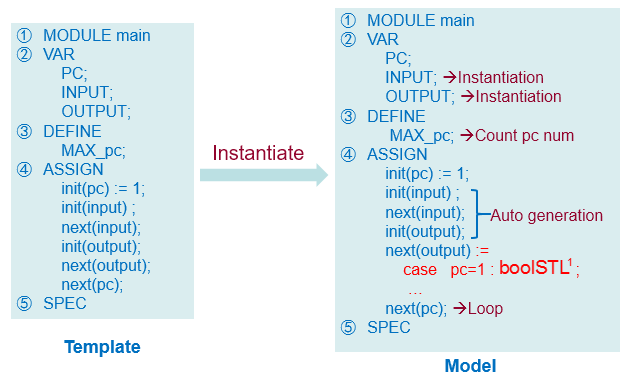
\includegraphics[scale=0.48]{spec/instantiation.png}
\caption{模板实例化过程}
\label{fig24}
\end{figure}

\subsection{模型检测}

由于PLC在每个执行周期使用状态变量来描述状态的变化。因此,我们仅分析单个执行周期来检查所有时间内的安全性规范是远远不够的。在本节中,我们将会给出了完整的模型检测算法来验证PLC程序的形式模型树图是否存在违反安全规范的路径。上一节提出的转换算法是对在所有执行周期里发生的状态变换进行建模并构建形式化模型的执行图,本节中我们采用CTL规范对模型进行验证并检测攻击,在更详细地阐述模型检测过程之前,我们简要介绍下用于安全规范的CTL。

\subsubsection{计算树逻辑CTL}

\textit {计算树逻辑},或简称CTL,是一个\textit {分支时间}逻辑,意味着它的时间模型是一个树状结构并且未来状态没有确定;在未来有不同的路径,任何一个都可能是实现的路径\parencite {klein2005fault}。

\textbf{定义 3}我们通过Backus Naur形式定义CTL公式:
\begin{equation} 
\begin{split}\phi :: = \bot | \top | p |(\neg\phi) | (\phi\wedge\phi) | (\phi\vee\phi) | (\phi\rightarrow\phi) | AX\phi |\\ EX\phi | AF\phi | EF\phi | AG\phi | EG\phi | A[\phi U \phi] | E[\phi U \phi]\end{split}
\end{equation}
这里\textit{p }是一组原子公式.

注意到每个CTL时间连接是一对符号,第一对是A和E之一。A意思是“沿所有路径”(\textit {不可避免}),E意思是“至少(存在)一个路径”(\textit {可能})。 第二对是X、F、G或U,分别表示“下一个状态”、“某些未来状态”、“所有未来状态(全局)”和“直到某个状态”。 例如,E[\textit{$\varphi{}$}$_{1 }$U \textit{$\varphi{}$}$_{2}$]中的符号对是EU。在CTL中,诸如EU的符号对是不可分割的。注意AU和EU是二进制的。符号X,F,G和U不能出现在A或E之前;类似地,每个A或E必须具有X,F,G和U中的一个。

\subsubsection{规范检测}

我们定义的过程安全规范是安全描述和控制系统与物理设备的约束行为。 基于规范的入侵检测尝试对控制逻辑模型$M$验证所有安全规范。如果发现反例,则给出可能存在恶意攻击注入智能控制器程序警报。

规范是由\textit {specifications}的有序列表组成且名称为\textit {id}的规范具有以下语法:
\[\begin{split}
id:  <input [input-list]> <output [output-list]> \\
<INIT [init-input-list]> <UNIQUE> \varphi
\end{split}
\]

例如,我们可以给出设备按钮的简单描述:“按下启动按钮时,原料M的阀门打开”,对应的规范如下面的\textit {lbutton}所示:
\[\raggedright
{ \textit{lbutton }: input~ \textit{launch}}{\small {^\ast} }{\large
~output~ \textit{v}_{M} ~INIT~ \textit{launch}}{\small {^\ast} }
\]

\[\raggedright
\textit{launch}^{*}\Rightarrow AX \textit{v}_{M}
\]

安全属性\textit {$ \phi {} $}在计算树逻辑(CTL)中的定义是规范唯一强制性的部分。CTL的规范定义的$ input $和$ output $来自控制程序的形式化模型集$ IO_\phi $,即$ \{input-list\} \cup{}  \{output-list\}$
$\subseteq{}$ \textit{$IO_\phi$}。验证过程分为三个步骤:基于规范的入侵检测将会通过控制逻辑模型$ M $验证\textit{$\phi{}$ }中的所有安全规范。
\begin{enumerate}
	\item 选择 $\phi$:~$\phi \leftarrow Pop(SPECs)$从安全规范集中$SPECs$取出一个属性$\phi$。
	\item 将形式化模型和物理设备变量的输入$input$和输出$output$映射集$IO_{M}$ 应用到$\phi$中. 定义为$\phi/IO_M$,即“在映射集$IO_M$下得到的属性$\phi$”。
	\item 验证 $M \vert{}$= \textit{$\phi/IO_M$}。
\end{enumerate}

这三个步骤适用于给定控制逻辑模型的所有安全规范,如算法\ref{algo:modelcheck}所示。首先,我们需要初始化输入和输出映射集$ IO_M $和控制逻辑模型$ M $,然后我们需要遍历安全规范$ SPECs $中的每个属性,并转换为$ IO_M $映射下的模型符号CTL规范。之后将通过MuSMV验证工具处理每个模型符号CTL规范$M \vert{}$= \textit{$\phi/IO_M$}。 如果存在不能通过模型检查并生成反例的任何属性,那么基于规范的入侵检测将激活警报机制,需要工作人员检查可能存在的某些注入当前系统程序的恶意代码。

\begin{algorithm}[h]
\caption{模型检测}
\label{algo:modelcheck}
\begin{algorithmic}[1]
\Require %算法的输入参数:Input  
安全 $SPECs$, 输入和输出映射集 $IO_M$和控制逻辑模型$M$ 

\Ensure %算法的输出:Output  
如果检测到存在攻击,则返回 $\mu_{CE}$并激活报警机制;否则返回安全通过; 
\State 初始化$IO_M$ 和 $M$
\For{each $\phi \in SPECs$}
\State $\phi \leftarrow IO_M$
\If { NOT $M \vert{}$= \textit{$\phi/IO_M$}}
\State $\mu_0 \leftarrow \textit{Counterexample Path}$
\State $\mu_{CE} \leftarrow \mu_{CE}\cup \mu_0$
\EndIf
\EndFor
\If {$\mu_{CE}.size() > 0$}
\State \textbf{激活} $alarm$
\EndIf
\State \textbf{return} $\mu_{CE}$

\end{algorithmic}
\end{algorithm}	

\section{实验仿真}
\label{sec:insertimage}

为了证明所提出的基于规范的检测方法的可行性和性能,我们给出了基于自动重合闸控制系统的仿真实验。该系统的功能是在瞬时故障发生时使用重合闸恢复电源,并在发生永久故障时使用备用电源。 该系统有9个输入(来自系统的测量)和11个输出(从PLC到执行器的信号)。 图\ref {fig29}显示了主电气连接图,图\ref {fig210}显示了系统的输入和输出映射表。

\begin{figure}[!htb]
\centering
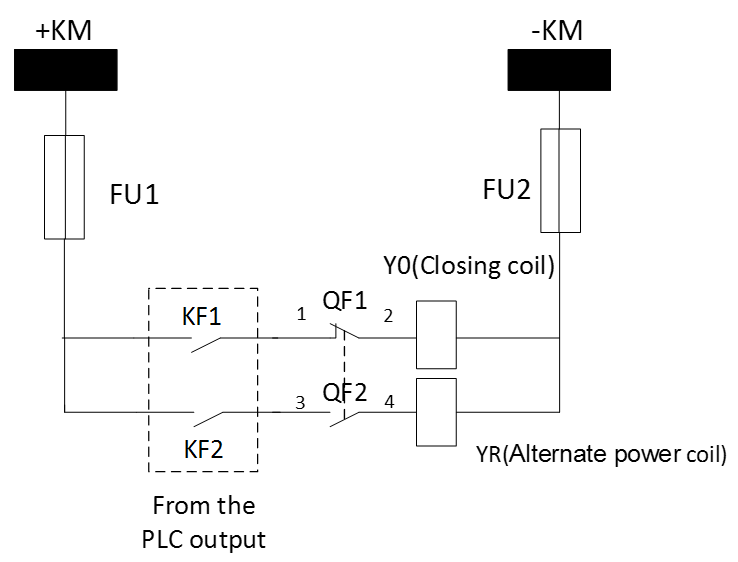
\includegraphics[scale=0.48]{spec/diagram.png}
\caption{自动重合闸控制系统主电气连接图}
\label{fig29}
\end{figure}

\begin{figure}[!htb]
\centering
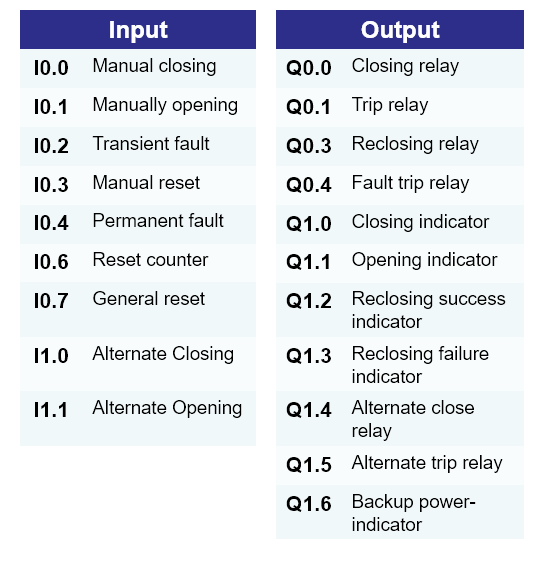
\includegraphics[scale=0.43]{spec/mappingTables.png}
\caption{自动重合闸控制系统的输入和输出映射表}
\label{fig210}
\end{figure}

首先,我们构建控制系统的形式模型,图\ref {fig211}显示了如何使用算法\ref{algo:boolil}将部分指令表程序去重处理并获得二进制函数输出进而转化为布尔逻辑指令表boolIL程序。图\ref {fig212}提供了NuSMV工具的实例化可执行代码模型的一部分,并且该模型应该写入以“.smv”结尾的文件。
\begin{figure}[!htb]{}
\centering
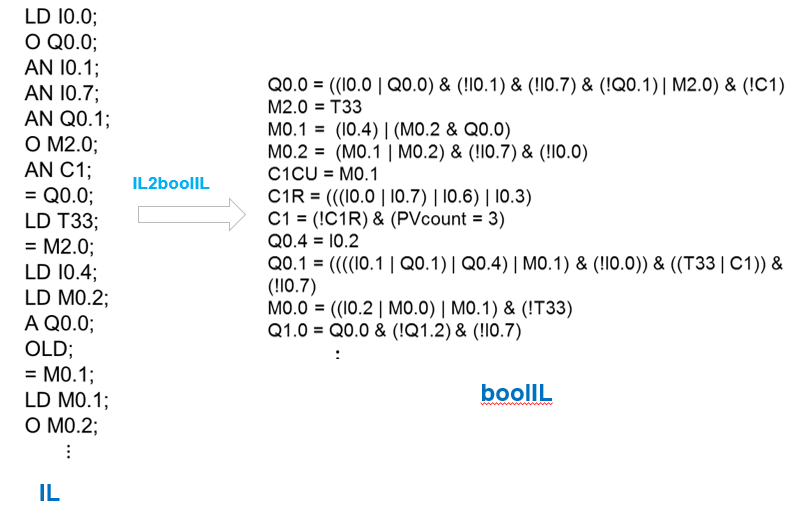
\includegraphics[scale=0.44]{spec/IL2boolIL.png}
\caption{IL2boolIL转化过程}
\label{fig211}
\end{figure}

\begin{figure}[!htb]
\centering
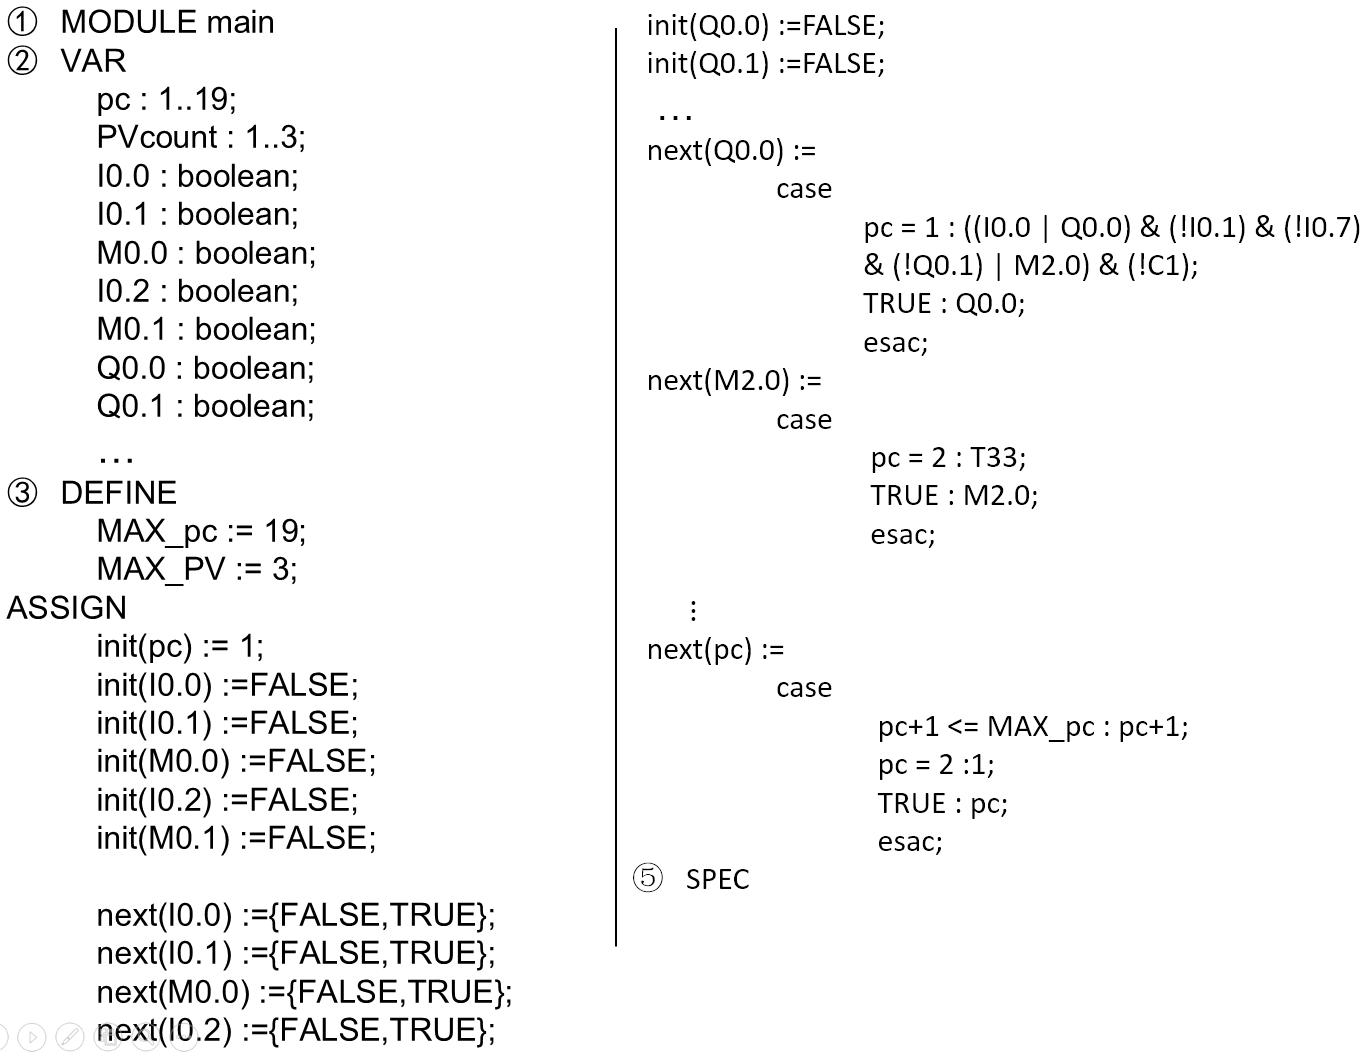
\includegraphics[scale=0.32]{spec/Instantiate.png}
\caption{实例化过程}
\label{fig212}
\end{figure}

为了使自动重合闸系统工作在预期的状态,我们为系统设计了7条主要的安全规范:
\begin{itemize}
	\item 关闭指示器在手动关闭回路时工作正常。
	\item 手动打开回路时,跳闸指示灯工作正常。
	\item 当模拟瞬态故障时,自动重合闸继电器工作且重合闸成功指示灯闪烁。
	\item 模拟永久故障时,自动重合闸继电器不工作且重合闸故障指示灯闪烁。
	\item 当模拟永久故障时,需要自动交流电源为用户提供电源,并且正在使用的备用电源指示灯可以顺利工作。
	\item 它可以手动关闭备用回路。
	\item 它可以手动打开交替回路。
\end{itemize}

在我们获得自动重合闸控制系统的程序模型后,我们需要构造CTL形式的规范。例如将第一个规范要求用形式化CTL规范可以得到:
\[\begin{split}
\bullet &AG(I\_ManualClosing\&(! I\_ManualOpening) )\&(! I\_GenReset) \\&-> AF(O\_ ClosingRelay));\\\bullet &AG((O\_ ClosingRelay \& (! I\_GenReset)) \\&-> AF(O\_ClosingIndicator));
\end{split}
\]

然而得到的规范都是由物理变量构成的,输入和输出映射表可以将物理变量替换成我们需要验证的程序变量。我们将根据映射中的\textit {input}和\textit {output}关键字之后给出的名称重新定义CTL的规范。 最终的CTL规格如下:
\[\begin{split}
\bullet &AG(I0.0\&(! I0.1) )\&(! I0.7) -> AF(O0.0));\\\bullet &AG((O0.0 \& (! I0.7)) -> AF(O1.0));
\end{split}
\]

类似地,其余的规范要求都可以转换为CTL规格。

如果没有对控制程序的任何攻击,在验证所有安全规范之后,每个规范将呈现“T”代表当前是安全状态。检测结果示于表\ref{spec:table3}。

\begin{table}[!htb]
\centering
\caption{未受到攻击时的验证结果}
\label{spec:table3}
\begin{tabular}{cccccccc}

\hline
Cycle & 1 & 2 & 3 & 4 & 5 & 6 & 7\\

1 & T & T & T & T & T & T & T\\

2 & T & T & T & T & T & T & T\\

3 & T & T & T & T & T & T & T\\

4 & T & T & T & T & T & T & T\\

~$\colon$ & ~$\colon$ & ~$\colon$ & ~$\colon$ & ~$\colon$ & ~$\colon$ & ~$\colon$ & ~$\colon$\\
\hline
\end{tabular}
\end{table} 

如果存在对控制程序的任何攻击,在验证所有安全规范之后,未能通过验证的安全属性将呈现“F”,意味着系统控制程序执行的结果与该安全规范相悖,系统正处于受攻击的不安全状态。检测结果如表\ref{spec:table4}所示。一旦面临这种情况,设备的相关攻击部分将立即发出报警并从可编程控制器中下载受感染程序,然后工程师需要根据验证结果检查第三和第六规格以修复控制系统。

\begin{table}[!htb]
\centering
\caption{存在攻击下的验证结果}
\label{spec:table4}
\begin{tabular}{cccccccc}

\hline
Cycle & 1 & 2 & 3 & 4 & 5 & 6 & 7\\

~$\colon$ & ~$\colon$ & ~$\colon$ & ~$\colon$ & ~$\colon$ & ~$\colon$ & ~$\colon$ & ~$\colon$\\

112 & T & T & F & T & T & F & T\\

113 & T & T & F & T & T & F & T\\

114 & T & T & F & T & T & F & T\\

~$\colon$ & ~$\colon$ & ~$\colon$ & ~$\colon$ & ~$\colon$ & ~$\colon$ & ~$\colon$ & ~$\colon$\\
\hline
\end{tabular}
\end{table} 

\section{本章小结}
\label{sec:insertimage}

在本章节中,我们提出了在过程控制系统中基于规范的入侵检测机制来应对可编程控制器程序被恶意代码注入攻击从而更好地保护过程控制系统。 我们给出了基于规范入侵检测的整个实现过程,包括对可编程控制器程序进行形式化建模。考虑到PLC程序的存在定时器和计数器等高级语言没有的指令,我们通过抽象建模给出等价的可执行二进制逻辑函数对其进行解释建模,这极大的增强了我们建模算法的通用性而不仅仅局限于基于运算指令。因为我们的检测对象是控制器本身包括控制程序和指令使其免受类似震网病毒的网络侵入和破坏。这可以确保控制器正确工作并保证上一章提出的基于异常数据检测的准确性和精度。最后基于自动重合闸控制系统的实验仿真表明,我们的检测能够对控制系统面临恶意代码注入的攻击威胁起到很好的保护作用并证明我们提出的方法的有效性。

